Esta tese tem como um dos objetivos a exportação de dados da \acrshort{api} de Classes (\acrshort{lc}), Entidades, Tipologias e Legislações em formato \acrshort{json}, \acrshort{xml} e \acrshort{csv}. Além disso, deve permitir a exportação da ontologia (possuidor da informação das variantes referidas a exportar) nos formatos \acrshort{rdf} seguintes: \acrshort{turtle}, \acrshort{json-ld} e \acrshort{rdf}/\acrshort{xml}.

A \acrshort{api} de dados já devolve a sua informação em \acrshort{json}. Portanto, por forma a realizar a exportação dos dados para outros formatos é necessário realizar a conversão de \acrshort{json} para o formato de saída pretendido.

Como tal, este capítulo inicia, no estado da arte, com a investigação de algumas bibliotecas disponíveis no \acrshort{npm} que têm como objetivo exportar de \acrshort{json} para \acrshort{xml} ou de \acrshort{json} para \acrshort{csv}.

\section{Estado da Arte}\label{sec:exportacao}

\subsection{\glsentryshort{xml}}

Comecemos por perceber o que é o \acrfull{xml}. Como se pode perceber pelo nome o \acrshort{xml} é uma linguagem \textit{Markup}, ou seja, uma linguagem que anota o texto para que a máquina possa manipular o texto de acordo com as anotações. O \acrshort{xml} foi desenhado para ser de fácil leitura tanto para humanos como para máquinas e tem como principal intuito o armazenamento e transporte de informação (o tal texto anotado). Além disso é extensível visto que permite que criemos as nossas \textit{tags}.

\begin{lstlisting}[language=xml, caption=Pequeno exemplo em \acrshort{xml}, label=exem:xmlEx]
<?xml version = "1.0" encoding = "UTF-8"?>
<pessoa>
    <nome>Maria</nome>
    <idade tipo="numero">23</idade>
    <morada>
        <pais>Portugal</pais>
        <cidade>Braga</cidade>
    </morada>
    <altura unidade="cm">160</altura>
    <!--Isto é um comentário-->
</pessoa>
\end{lstlisting}

De seguida serão apresentadas, de forma simplificada, as regras de sintaxe aplicadas ao \acrshort{xml} para cada componente deste.

\begin{itemize}
    \item \textbf{Declaração \acrshort{xml}} \\
    \verb|<?xml version = "1.0" encoding = "UTF-8"?>| \\
    Opcional, especifica a versão do \acrshort{xml} e o \textit{encoding} usado no documento
    \begin{itemize}
        \item A declaração é \textit{case-sensitive} pelo que deve começar obrigatoriamente por \texttt{xml}
        \item Se presente no documento, a declaração tem de ser obrigatoriamente o primeiro componente
    \end{itemize}
    \item \textbf{\textit{Tags} e elementos} \\
    \verb|<nome>Maria</nome>| ou \verb|<semnome/>|
    \begin{itemize}
        \item Cada elemento tem de ser fechado seja por uma \textit{tag} (\textit{tag} final), ou como apresentado acima pela própria \textit{tag}.
        \item Os elementos \acrshort{xml} podem conter elementos filhos mas estes não se podem sobrepor, ou seja, uma \textit{tag} final de um elemento tem de ter o mesmo nome que a última \textit{tag} inicial ainda sem \textit{tag} final. 
        \item Um documento \acrshort{xml} apenas pode ter um elemento na raiz do documento (elemento \textit{root})
        \item Os nomes das \textit{tags} são \textit{case-sensitive}, portanto, a \textit{tag} inicial e final de um elemento têm de ser exatamente iguais
    \end{itemize}
    \item \textbf{Atributos} \\
    \verb|<altura unidade="cm">160</altura>| \\
    onde `unidade' é o nome do atributo e `cm' é o valor do atributo. Um atributo especifica uma propriedade de um elemento
    \begin{itemize}
        \item Um elemento pode ter zero, um ou mais atributos
        \item Os nomes dos atributos são \textit{case-sensitive}
        \item Um atributo não pode ter dois valores num elemento, ou seja, não pode ser declarado duas ou mais vezes num mesmo elemento
        \item Os nomes dos atributos não podem possuir aspas, mas os valores tem de ser encapsulados por aspas
    \end{itemize}
    \item \textbf{Referências \acrshort{xml}} \\
    \verb|&amp;| ou \verb|&#65| \\
    Há dois tipos de referências, Referências Entidade ou Referências Caractere. A primeira existe por forma a serem representadas por estas referências os caracteres não permitidos no texto anotado visto representarem parte da sintaxe do \acrshort{xml}.
    \begin{center}
        \begin{tabular}{|c|c|}
            \hline
            Caractere não permitido & Entidade \\ \hline
            < & \&lt; \\ \hline
            > & \&gt; \\ \hline
            \& & \&amp; \\ \hline
            ' & \&apos; \\ \hline
            " & \&quot; \\ \hline
        \end{tabular}
    \end{center}
    O segundo tipo de referências tem o mesmo intuito mas permite que seja representado qualquer caractere representável em \textit{Unicode}. O número que se segue ao \textit{hashtag} é referente ao código decimal em \textit{Unicode}. Assim \verb|&#65| representa o caractere `A'.
    \item \textbf{Texto anotado} \\
    Espaços em branco, \textit{tabs}, ou novas linhas, são ignoradas quando presentes entre elementos e entre atributos. Como já referido há caracteres reservados pelo que se pretende usá-los no texto anotado deve trocar esses caracteres pelas suas referências.
\end{itemize}

\subsubsection{Bibliotecas de conversão}

Nesta secção serão abordadas algumas bibliotecas de conversão de \acrshort{json} para \acrshort{xml}, aquelas com maior popularidade e adesão no \acrshort{npm}.

Por forma a ter uma ideia do resultado devolvido por cada biblioteca será usado o seguinte exemplo:
\begin{lstlisting}[language=json, caption=Exemplo em \acrshort{json} a converter, label=exem:jsonBib]
[
    {
        "nome": "Maria",
        "idade": "22",
        "morada": {
            "pais": "Portugal",
            "cidade": "Braga"
        }
    },
    {
        "nome": "João",
        "idade": "24",
        "morada": {
            "pais": "Portugal",
            "cidade": "Vila Real"
        }
    }
]
\end{lstlisting}

\paragraph{\href{https://www.npmjs.com/package/xml-js}{\texttt{xml-js}}} \mbox{} \\

Esta biblioteca permite a conversão nos dois sentidos, ou seja, de \acrshort{json} para \acrshort{xml} e de \acrshort{xml} para \acrshort{json}.

As principais características que esta biblioteca possui para uma conversão de \acrshort{json} para \acrshort{xml} são:
\begin{itemize}
    \item Mantém a ordem dos elementos
    \item Totalmente compatível com \acrshort{xml}
    \item Reversível, é possível reverter o resultado para o original
    \item Podem ser fornecidas funções personalizadas para processamento adicional para diferentes partes do \acrshort{xml} ou do \acrshort{json} a converter
\end{itemize}

\begin{lstlisting}[language=xml, caption=Resultado da conversão do exemplo~\ref{exem:jsonBib} usando o conversor \texttt{xml-js}]
<0>
    <nome>Maria</nome>
    <idade>22</idade>
    <morada>
        <pais>Portugal</pais>
        <cidade>Braga</cidade>
    </morada>
</0>
<1>
    <nome>João</nome>
    <idade>24</idade>
    <morada>
        <pais>Portugal</pais>
        <cidade>Vila Real</cidade>
    </morada>
</1>
\end{lstlisting}

\paragraph{\href{https://www.npmjs.com/package/xmlbuilder}{\texttt{xmlbuilder}}} \mbox{} \\

A biblioteca tem como intuito principal a construção de documentos \acrshort{xml} através do uso de funções, como se pode comprovar de seguida:

\begin{lstlisting}[language=javascript, caption=Código para a construção em \acrshort{xml} do exemplo~\ref{exem:xmlEx} usando o \texttt{xmlbuilder}]
var builder = require('xmlbuilder');
 
var xml = builder.create('pessoa')
    .ele('nome', 'Maria')
    .up()
    .ele('idade', {'tipo': 'numero'}, '23')
    .up()
    .ele('morada')
    .ele('pais', 'Portugal')
    .up()
    .ele('cidade', 'Braga')
    .up()
    .up()
    .ele('altura', {'unidade': 'cm'}, '160')
    .up()
    .com('Isto é um comentário')
    .end({ pretty: true});
\end{lstlisting}

Além disso, permite a geração do \acrshort{xml} a partir de um objeto \acrshort{json} o que permite, como tal, a conversão de \acrshort{json} para \acrshort{xml} que se necessita.

\begin{lstlisting}[language=xml, caption=Resultado da conversão do exemplo~\ref{exem:jsonBib} usando o conversor \texttt{xmlbuilder}]
<?xml version="1.0" encoding="utf-8"?>
<nome>Maria</nome>
<idade>22</idade>
<morada>
  <pais>Portugal</pais>
  <cidade>Braga</cidade>
</morada>
<nome>João</nome>
<idade>24</idade>
<morada>
  <pais>Portugal</pais>
  <cidade>Vila Real</cidade>
</morada>
\end{lstlisting}

Na construção do documento a partir de um objecto, quando se pretende que um elemento tenha um atributo, é necessário que o objeto para essa chave possua um objeto em vez de apenas o valor. Nesse objeto, as propriedades começadas por `@' indicam atributos (\verb|'@unidade':'cm'| onde `unidade' é o nome do atributo e `cm' é o valor do atributo) e a propriedade '\#text' representa o valor do elemento.

Há também a possibilidade de sobrescrever as funções usadas para escrever o documento \acrshort{xml} (funções de escrita dos elementos, comentários, etc) bem como as funções que convertem os valores (texto anotado, nome de elementos e atributos, etc).

Por fim, convém referir que esta biblioteca já possui uma sucessora, \href{https://www.npmjs.com/package/xmlbuilder2}{\texttt{xmlbuilder2}}, que foi redesenhada por forma a estar em total conformidade com a especificação moderna do \acrshort{dom}.

\paragraph{\href{https://www.npmjs.com/package/xml2js}{\texttt{xml2js}}} \mbox{} \\

De igual forma como a biblioteca \texttt{xml-js}, esta biblioteca consegue converter de \acrshort{json} para \acrshort{xml} como de \acrshort{xml} para \acrshort{json}. 

\begin{lstlisting}[language=xml, caption=Resultado da conversão do exemplo~\ref{exem:jsonBib} usando o conversor \texttt{xml2js}]
<?xml version="1.0" encoding="UTF-8" standalone="yes"?>
<root>
  <nome>Maria</nome>
  <idade>22</idade>
  <morada>
    <pais>Portugal</pais>
    <cidade>Braga</cidade>
  </morada>
  <nome>João</nome>
  <idade>24</idade>
  <morada>
    <pais>Portugal</pais>
    <cidade>Vila Real</cidade>
  </morada>
</root>
\end{lstlisting}

Se se pretende que um determinado elemento possua atributos é necessário que o objeto para esse elemento seja um objeto (\verb|{$: {unidade: 'cm'}, _: '160'}|) onde `\_' é o texto anotado e os vários atributos devem estar no objeto da propriedade `\$' em que o nome da propriedade é o nome do atributo e o valor da propriedade é o valor do atributo.

\subsection{\glsentryshort{csv}}

\acrfull{csv} como a sua sigla indica é um documento em que os campos de um registo são separados por uma vírgula. Contudo, os campos não precisam de ser obrigatoriamente separados por vírgula já que podem também ser separados por ponto e vírgula, \textit{tabs}, \textit{pipes} (`|') ou ainda outro qualquer caractere que se pretenda usar. Quando se usa o caractere separador ou uma nova linha (`\backslash{}n') no campo de um registo, por forma a não ser considerado como um separador de campos ou de registos respetivamente, pode-se encapsular os valores por aspas (`"') sendo que também se pode usar outro caractere em vez das aspas. Já quando se usa o caractere de encapsulamento no campo de um registo este deve ser protegido (\texttt{escaped}) repetindo o mesmo caractere de encapsulamento.

Um documento \acrshort{csv} é nada mais que uma tabela que guarda dados em texto. É usado essencialmente para a troca de dados.

Após esta pequena introdução ao \acrshort{csv} apresenta-se as regras de sintaxe para a criação de um documento \acrshort{csv}:
\begin{itemize}
    \item Campos separados com um separador, normalmente uma vírgula
    \item Cada registo deve estar numa linha. Cada registo deve começar numa linha, mas cada registo pode ter várias linhas, desde que os campos multi linha sejam encapsulados por aspas
    \item Após o último registo não deve estar presente um \textit{carriage return}
    \item Opcionalmente, na primeira linha do documento, deve estar presente o cabeçalho com os nomes das colunas separados pelo separador usado no resto do documento
    \item O caractere de encapsulamento deve ser usado para encapsular um campo quando necessário (pode ser usado sempre), isto é, quando o caractere separador ou uma nova linha (`\backslash{}n') são usados num campo de um registo
\end{itemize}

\begin{lstlisting}[caption=Pequeno exemplo em \acrshort{csv}, label=exem:csvEx]
Nome,Idade,País,Cidade,Altura
"Silva, Maria",23,Portugal,Braga,160cm
\end{lstlisting}

\subsubsection{Bibliotecas de conversão}

Nesta secção irá também ser aprofundada algumas bibliotecas de conversão de \acrshort{json} para \acrshort{csv}, aquelas com maior popularidade no \acrshort{npm}.

\paragraph{\href{https://www.npmjs.com/package/papaparse}{\texttt{papaparse}}} \mbox{} \\

O \texttt{papaparse} tem como principal objetivo realizar o \textit{parse} de ficheiros \acrshort{csv}. Consegue contudo reverter, convertendo de \acrshort{json} para \acrshort{csv}.

\begin{lstlisting}[caption=Resultado da conversão do exemplo~\ref{exem:jsonBib} usando o conversor \texttt{papaparse}, label=exem:papaparse]
nome,idade,morada
Maria,22,[object Object]
João,24,[object Object]
\end{lstlisting}

Olhando para o resultado~\ref{exem:papaparse} consegue-se perceber que o conversor não consegue converter objetos aninhados. Para além disso, apesar de haver a possibilidade de alterar o caractere separador, o caractere de \textit{escape}, o caractere de nova linha bem como definir o nome das colunas no cabeçalho, não é possível definir uma função por forma a alterar a conversão dos campos de cada propriedade.

\paragraph{\href{https://www.npmjs.com/package/json2csv}{\texttt{json2csv}}} \mbox{} \\

Biblioteca totalmente dedicada à conversão de \acrshort{json} para \acrshort{csv}. Tem como principais características:
\begin{itemize}
    \item Permite a alteração dos caracteres de separação, de encapsulamento e de nova linha
    \item \textit{Escape} automático
    \item Permite escolher que campos devolver (mesmo em objetos aninhados ou listas aninhadas) e que cabeçalho associar a cada campo
    \item Aceita funções de transformação para cada campo
\end{itemize}

\begin{lstlisting}[caption=Resultado da conversão do exemplo~\ref{exem:jsonBib} usando o conversor \texttt{json2csv}, label=exem:json2csv]
"nome","idade","morada.pais","morada.cidade"
"Maria","22","Portugal","Braga"
"João","24","Portugal","Vila Real"
\end{lstlisting}

Para além disso permite o \textit{unwind} de uma propriedade que possua uma lista, fazendo com que sejam gerados x registos de acordo com o tamanho da lista, sendo alterado apenas os valores que provêm da lista. Infelizmente isto acrescenta mais colunas, não permitindo que no caso de os elementos da lista (filhos) tenham a mesma estrutura que o pai, sejam adicionados como novos registos, sem adicionar novas colunas e sem repetir a informação do pai. 

Por exemplo, se pretendermos converter o seguinte documento \acrshort{json}:
\begin{lstlisting}[language=json, caption=Outro exemplo em \acrshort{json} a converter, label=exem:jsonBib2]
[
    {
        "nome": "Maria",
        "idade": "22",
        "morada": {
            "pais": "Portugal",
            "cidade": "Braga"
        },
        "filhos": [
          {
            "nome": "António",
            "idade": "2",
            "morada": {
                "pais": "Portugal",
                "cidade": "Braga"
            }
          }
        ]
    },
    {
        "nome": "João",
        "idade": "24",
        "morada": {
            "pais": "Portugal",
            "cidade": "Vila Real"
        },
        "filhos": []
    }
]
\end{lstlisting}

Usando este conversor é possível obter:
\begin{lstlisting}[caption=Resultado da conversão do exemplo~\ref{exem:jsonBib2} usando o conversor \texttt{json2csv}]
"nome","idade","morada.pais","morada.cidade","filhos.nome","filhos.idade","filhos.morada.pais","filhos.morada.cidade"
"Maria","22","Portugal","Braga","António","2","Portugal","Braga"
"João","24","Portugal","Vila Real",,,,
\end{lstlisting}

Quando o resultado pretendido seria por exemplo:
\begin{lstlisting}[caption=Resultado pretendido da conversão do exemplo~\ref{exem:jsonBib2}]
"nome","idade","morada.pais","morada.cidade"
"Maria","22","Portugal","Braga",
"António","2","Portugal","Braga"
"João","24","Portugal","Vila Real"
\end{lstlisting}

\subsection{Ontologia}

\subsubsection{O que é uma ontologia?}

Uma ontologia é uma descrição formal e explícita de conceitos num domínio de discurso (classes, chamado às vezes de conceitos), propriedades de cada conceito que descrevem várias características e atributos do conceito (\textit{slots}, às vezes chamados de funções ou propriedades) e restrições sobre \textit{slots} (facetas, às vezes chamadas de restrições de função).~\cite{ontologyProt} Uma ontologia, juntamente com um conjunto de instâncias individuais de classes, constitui uma base de conhecimento.~\cite{ontologyProt}

Uma ontologia pode ser dividida em duas partes:
\begin{itemize}
    \item Estrutura: Onde é definido as classes, as propriedades (\textit{slots}) e as restrições das propriedades (facetas)
    \item População: Onde é definido indivíduos (de classes) e propriedades dos indivíduos. Esta parte é construída tendo por base a estrutura definida.
\end{itemize}
De certa forma, a estrutura é como se fosse o modelo definido e a população a informação guardada respeitando o modelo definido.

Falemos agora um pouco mais sobre cada componente de uma ontologia.

Começando pelas classes, estas correspondem a conceitos, sendo que uma classe pode ter subclasses (onde uma subclasse herda as propriedades da sua superclasse) e superclasses. Para além disso, as classes possuem instâncias (ou indivíduos). Quanto às propriedades das classes existem dois tipos:
\begin{itemize}
    \item Atributos: propriedade que permite definir uma característica de uma classe (ou indivíduo) (p.e: Se pessoa for uma classe, o nome será um atributo)
    \item Relações: propriedade que permite estabelecer relações entre classes (ou indivíduos) (p.e: A relação de pai entre duas pessoas) 
\end{itemize}

As próprias propriedades podem ser caracterizadas através das restrições. As principais restrições são:
\begin{itemize}
    \item Cardinalidade: Indica quantos valores pode ter uma propriedade, \texttt{0} a \texttt{n} (p.e: Uma pessoa só tem um pai biológico.; outro exemplo: Uma pessoa pode ter várias nacionalidades)
    \item Tipo de valor: Indica que tipo de valor terá a propriedade (atributo), \textit{string}, número, \textit{boolean}, etc (p.e: A idade de uma pessoa é um número; outro exemplo: O nome de uma pessoa é uma \textit{string})
    \item \textit{Domain} e \textit{Range}: Indica que tipo de instâncias podem ser relacionadas por uma propriedade. O \textit{Domain} indica a quem pertence a propriedade (atributo ou relação). Já o \textit{Range} indica para uma relação o tipo de instâncias que podem ser relacionadas com o \textit{Domain} (p.e: Na relação pai, o seu \textit{Domain} e o seu \textit{Range} são iguais a Pessoa.; outro exemplo: Seja Animal outra classe, a relação tem dono tem como \textit{Domain} Animal e como \textit{Range} Pessoa; ainda outro exemplo: O \textit{Domain} do atributo nome é Pessoa)
\end{itemize}

\subsubsection{\textit{Web} Semântica}

A \textit{web} semântica é uma extensão da \acrshort{www} com o objetivo de tornar a informação da internet legível por máquinas (\textit{machine-readable}).

Para isso a \acrfull{w3c} está a ajudar a criar a \textit{stack} tecnológica necessária. O termo \textit{web} semântica é a visão da \acrshort{w3c} acerca da \textit{Linked Data} na \textit{Web}, ou seja, é a web dos dados em que a coleção de tecnologias da \textit{web} semântica (\acrshort{rdf}, \acrshort{sparql}, \acrshort{owl}, \acrshort{skos}, etc) oferece um ambiente onde as pessoas podem criar bases de dados na \textit{web}, construir ontologias e escrever regras para manipular os dados; e onde as aplicações podem questionar esses dados e desenhar inferências usando vocabulários.

Para tornar a \textit{web} dos dados uma realidade é necessário existir uma grande quantidade de dados na \textit{web} num formato \textit{standard} (\acrshort{rdf}), acessível e gerível pelas ferramentas da \textit{web} semântica. Além disso, a \textit{web} semântica necessita também que existam relações entre os dados para criar a \textit{web} dos dados (\textit{Linked Data}). É também importante ser possível configurar \textit{query endpoints} para aceder aos dados mais convenientemente. A \acrshort{w3c} fornece uma palete de tecnologias, das quais se destaca o \acrshort{sparql}, para obter acesso aos dados.

A \textit{Linked Data} é usada para a integração em grande escala e o \textit{reasoning}\footnote{Em \textit{web} semântica é a inferência de informação (triplos) a partir de um conjunto de factos (triplos), ou seja, a descoberta de novos factos (triplos)} dos dados na \textit{web}.

Na \textit{web} semântica, os vocabulários definem os conceitos e os relacionamentos usados para descrever e representar uma área de interesse. Não há uma divisão clara entre o que é referido como ``vocabulários'' e ``ontologias''. A tendência é usar a palavra ``ontologia'' para coleções de termos mais complexos e mais formais, enquanto que ``vocabulário'' nas coleções menos formais. A \acrshort{w3c} oferece várias técnicas para descrever e definir diferentes formas de vocabulários num formato \textit{standard}. Estas incluem \acrshort{rdf} e \acrshort{rdf} Schemas, \acrshort{skos}, \acrshort{owl} e \acrshort{rif}. A escolha da tecnologia depende da complexidade e do rigor necessário.

Tal como as bases de dados relacionais ou o \acrshort{xml} necessitam de linguagens de pesquisa (\textit{query}) específicas (\acrshort{sql} e \textit{XQuery}, respetivamente), a \textit{web} dos dados, tipicamente representada usando \acrshort{rdf} como formato de dados, necessita também de uma linguagem de pesquisa. Isto é providenciado pelo \acrshort{sparql}, que é também um protocolo de comunicação, permitindo enviar \textit{queries} e receber resultados, por exemplo, através de \acrshort{http} ou \acrshort{soap}.

As \textit{queries} \acrshort{sparql} são baseadas em padrões (triplos). O \acrshort{rdf} pode ser visto como um conjunto de relacionamentos entre recursos (triplos \acrshort{rdf}). As \textit{queries} \acrshort{sparql} possuem um ou mais padrões semelhantes aos triplos \acrshort{rdf}, exceto que um ou mais dos recursos constituintes referenciados são variáveis. Um motor \acrshort{sparql} retornará os recursos que para todos os triplos correspondem a esses padrões. A informação devolvida pelos \textit{endpoints} \acrshort{sparql} pode ser uma tabela ou por exemplo \acrshort{json}.

\subsubsection{\textit{GraphDB}}

O \textit{GraphDB} é uma \acrfull{bd} Semântica baseada em grafos compatível com os padrões \acrshort{w3c}. É a base de dados principal quando se pretende trabalhar com a \textit{web} semântica. Suporta \acrshort{rdf} e \acrshort{sparql} e possui funcionalidades de exportação dos triplos presentes numa \acrshort{bd} armazenada no \textit{GraphDB}.

Para um fácil uso e compatibilidade com os \textit{standards} da indústria, o \textit{GraphDB} implementou as interfaces da \textit{framework} \textit{RDF4J}, a especificação do protocolo \acrshort{w3c} \acrshort{sparql}\footnote{Ver \url{https://www.w3.org/TR/sparql11-protocol/}} e suporta vários formatos de serialização \acrshort{rdf}\footnote{\label{fnRDF}\textit{TriG}, \textit{BinaryRDF}, \textit{TriX}, \textit{N-Triples}, \textit{N-Quads}, \acrshort{n3}, \acrshort{rdf}/\acrshort{xml}, \acrshort{rdf}/\acrshort{json}, \acrshort{json-ld} e \acrshort{turtle}}.~\cite{graphdbAbout}

O \textit{GraphDB} é um \textit{plugin} \acrshort{sail} para a \textit{framework} \textit{RDF4J} fazendo uso extensivo dos recursos e infraestrutura do \textit{RDF4J} especialmente do modelo \acrshort{rdf}, dos \textit{parsers} \acrshort{rdf} e dos motores de pesquisa.~\cite{graphdbArch}

Assim, o \textit{GraphDB} possui uma \acrshort{rest} \acrshort{api} do servidor \textit{RDF4J}\footnote{Ver \url{https://rdf4j.org/documentation/rest-api/}} a partir da qual é possível obter todos os triplos de uma \acrshort{bd} através da rota
\begin{verbatim}
<url do GraphDB>/repositories/<id do repositório (BD)>/statements
\end{verbatim}
indicando no cabeçalho \acrshort{http} \textit{Accept} o formato de serialização \acrshort{rdf}\footnoteref{fnRDF} de saída (\textit{\acrshort{mime} type}\footnote{\textit{Standard} que indica a natureza e o formato de um documento, ficheiro ou conjunto de \textit{bytes}. Ver \href{https://tools.ietf.org/html/rfc6838}{RFC 6838}}) dos triplos.

\section{Solução}

Nesta secção será apresentado a especificação dos documentos finais das exportações a realizar, 
decidindo se algumas das bibliotecas apontadas no estado da arte (\ref{sec:exportacao}) permitem auxiliar 
ou realizar as conversões necessárias.

\subsection{\glsentryshort{xml}}

De seguida, apresenta-se a especificação do documento final em \acrshort{xml}:
\begin{itemize}
    \item Os dados exportados devem ser encapsulados com a \textit{tag} \texttt{root} por forma a garantir que 
    só existe um elemento \textit{root} no documento \acrshort{xml} gerado respeitando as regras do \acrshort{xml}
    \item Cada tipo de dados do \acrshort{json} deve ser convertido da seguinte forma:
    \begin{itemize}
        \item \textit{string}: Mantém-se igual tirando os caracteres ``\texttt{<}'', ``\texttt{>}'', 
        ``\texttt{\&}'', ``\texttt{'}'' e ``\texttt{"}'' que devem ser convertidos para a 
        \textit{Entity Reference}\footnote{``\texttt{<}'' para ``\texttt{\&lt;}'', ``\texttt{>}'' 
        para ``\texttt{\&gt;}'', ``\texttt{\&}'' para ``\texttt{\&amp;}'', ``\texttt{'}'' para ``\texttt{\&apos;}'' 
        e ``\texttt{"}'' para ``\texttt{\&quot;}''} correspondente;
        \item \textit{number}: Mantém-se igual;
        \item \textit{boolean}: Mantém-se igual;
        \item \textit{null}: Origina uma \textit{string} vazia;
        \item \textit{array}: Cada item do \textit{array} deve ser encapsulado numa \textit{tag} \texttt{item} 
        que possui um atributo \texttt{index} que indica a posição do elemento no \textit{array} e um atributo 
        \texttt{type} que indica o tipo do elemento do \textit{array}. O tipo pode ser \textit{number}, 
        \textit{boolean}, \textit{string}, \textit{array} ou \textit{object};
        \item \textit{object}: Para cada propriedade deve ser criado uma \textit{tag} com valor igual à chave da 
        propriedade e ao valor da propriedade deve ser aplicado recursivamente uma das transformações desta lista. 
        Esta \textit{tag} deve ter um atributo \texttt{type} em que o seu valor, tal como nos \textit{arrays}, 
        pode ser \textit{number}, \textit{boolean}, \textit{string}, \textit{array} ou \textit{object}.
    \end{itemize}
\end{itemize}

Depois de compreendida a especificação, se observarmos as bibliotecas exploradas na secção do estado da arte,
percebemos que não há nenhuma que permita obter esta especificação sem alterar o objeto \acrshort{json} a 
exportar (a converter) o que acaba por em certas situações ser mais complicado do que construir um conversor 
específico para esta especificação. Assim, decidiu-se que seria criado um conversor de \acrshort{json} para 
\acrshort{xml}.

\subsection{\glsentryshort{csv}}

O documento \acrshort{csv} exportado deve respeitar a seguinte especificação:
\begin{itemize}
    \item O conjunto de objetos permitidos é lista de classes, de entidades, de tipologias e de legislações 
    e objeto de classe, de entidade, de tipologia e de legislação;
    \item A conversão das listas de classes, de entidades, de tipologias e de legislações deve ter a presença 
    dos títulos na primeira linha e depois um elemento por linha;
    \item Todos os valores das propriedades tem de ser encapsulados com aspas (\verb|"|);
    \item Os valores de uma linha devem ser concatenados com ponto e vírgula (\verb|;|);
    \item As linhas devem ser concatenadas com nova linha (\verb|\n|);
    \item Caso o valor de uma propriedade a converter seja uma lista, a conversão a realizar irá depender da 
    propriedade e do objeto que está a ser convertido: 
    \begin{itemize}
        \item Num objeto Classe:
        \begin{itemize}
            \item Propriedade `notasAp':
            \begin{itemize}
                \item Título: Notas de aplicação \\
                      Valor: Concatenação por \verb|#\n| da propriedade `nota' de cada elemento da lista
            \end{itemize}
            \item Propriedade `exemplosNotasAp':
            \begin{itemize}
                \item Título: Exemplos de NA \\
                      Valor: Concatenação por \verb|#\n| da propriedade `exemplo' de cada elemento da lista
            \end{itemize}
            \item Propriedade `notasEx':
            \begin{itemize}
                \item Título: Notas de exclusão \\
                      Valor: Concatenação por \verb|#\n| da propriedade `nota' de cada elemento da lista
            \end{itemize}
            \item Propriedade `termosInd':
            \begin{itemize}
                \item Título: Termos Indice \\
                      Valor: Concatenação por \verb|#\n| da propriedade `termo' de cada elemento da lista
            \end{itemize}
            \item Propriedade `donos':
            \begin{itemize}
                \item Título: Donos do processo \\
                      Valor: Concatenação por \verb|#\n| da propriedade `sigla' de cada elemento da lista
            \end{itemize}
            \item Propriedade `participantes', gera duas colunas no \acrshort{csv}:
            \begin{itemize}
                \item Título: Participante no processo \\
                      Valor: Concatenação por \verb|#\n| da propriedade `sigla' de cada elemento da lista
                \item Título: Tipo de intervenção do participante \\
                      Valor: Concatenação por \verb|#\n| da propriedade `participLabel' de cada elemento da lista
            \end{itemize}
            \item Propriedade `processosRelacionados', gera três colunas no \acrshort{csv}:
            \begin{itemize}
                \item Título: Código do processo relacionado \\
                      Valor: Concatenação por \verb|#\n| da propriedade `codigo' de cada elemento da lista
                \item Título: Título do processo relacionado \\
                      Valor: Concatenação por \verb|#\n| da propriedade `titulo' de cada elemento da lista
                \item Título: Tipo de relação entre processos \\
                      Valor: Concatenação por \verb|#\n| da propriedade `idRel' de cada elemento da lista
            \end{itemize}
            \item Propriedade `legislacao', gera duas colunas no \acrshort{csv}:
            \begin{itemize}
                \item Título: Diplomas jurídico-administrativos REF Ids \\
                      Valor: Concatenação por \verb|#\n| da propriedade `idLeg' de cada elemento da lista
                \item Título: Diplomas jurídico-administrativos REF Títulos \\
                      Valor: Cada elemento da lista é mapeado para a concatenação da propriedade `tipo' com a propriedade `numero' com um espaço entre as duas propriedades; Concatenação por \verb|#\n| do mapeamento de cada elemento da lista
            \end{itemize}
            \item Propriedade `filhos': cada elemento deve ser convertido como se tratasse de um objeto classe; 
            Devem ser ignorados os títulos gerados, mantendo apenas os valores numa nova linha do \acrshort{csv}.
        \end{itemize}
        \item Num objeto Entidade:
        \begin{itemize}
            \item Propriedade `dono':
            \begin{itemize}
                \item Título: Dono no processo \\
                      Valor: Concatenação por \verb|#\n| da propriedade `codigo' de cada elemento da lista
            \end{itemize}
            \item Propriedade `participante', gera duas colunas no \acrshort{csv}:
            \begin{itemize}
                \item Título: Participante no processo \\
                      Valor: Concatenação por \verb|#\n| da propriedade `codigo' de cada elemento da lista
                \item Título: Tipo de intervenção no processo \\
                      Valor: Concatenação por \verb|#\n| da propriedade `tipoPar' de cada elemento da lista
            \end{itemize}
            \item Propriedade `tipologias':
            \begin{itemize}
                \item Título: Tipologias da entidade \\
                      Valor: Concatenação por \verb|#\n| da propriedade `sigla' de cada elemento da lista
            \end{itemize}
        \end{itemize}
        \item Num objeto Tipologia:
        \begin{itemize}
            \item Propriedade `entidades':
            \begin{itemize}
                \item Título: Entidades da tipologia \\
                      Valor: Concatenação por \verb|#\n| da propriedade `sigla' de cada elemento da lista
            \end{itemize}
            \item Propriedade `dono':
            \begin{itemize}
                \item Título: Dono no processo \\
                      Valor: Concatenação por \verb|#\n| da propriedade `codigo' de cada elemento da lista
            \end{itemize}
            \item Propriedade `participante', gera duas colunas no \acrshort{csv}:
            \begin{itemize}
                \item Título: Participante no processo \\
                      Valor: Concatenação por \verb|#\n| da propriedade `codigo' de cada elemento da lista
                \item Título: Tipo de intervenção no processo \\
                      Valor: Concatenação por \verb|#\n| da propriedade `tipoPar' de cada elemento da lista
            \end{itemize}
        \end{itemize}
        \item Num objeto Legislação:
        \begin{itemize}
            \item Propriedade `entidades':
            \begin{itemize}
                \item Título: Entidades \\
                      Valor: Concatenação por \verb|#\n| da propriedade `sigla' de cada elemento da lista
            \end{itemize}
            \item Propriedade `regula':
            \begin{itemize}
                \item Título: Regula processo \\
                      Valor: Concatenação por \verb|#\n| da propriedade `codigo' de cada elemento da lista
            \end{itemize}
        \end{itemize}
        \item Na propriedade `pca' de um objeto Classe:
        \begin{itemize}
            \item Propriedade `justificacao', gera duas colunas no \acrshort{csv}:
            \begin{itemize}
                \item Título: Critério PCA \\
                      Valor: Concatenação por \verb|#\n| da propriedade `tipoId' de cada elemento da lista
                \item Título: ProcRefs/LegRefs PCA \\
                      Valor: Cada elemento da lista é mapeado para a concatenação por \verb|#\n| da lista presente na propriedade `processos' ou na propriedade `legs' sendo a concatenação encapsulada por parênteses curvos; Concatenação por \verb|#\n| do mapeamento de cada elemento da lista               
            \end{itemize}
        \end{itemize}
        \item Na propriedade `df' de um objeto Classe:
        \begin{itemize}
            \item Propriedade `justificacao', gera duas colunas no \acrshort{csv}:
            \begin{itemize}
                \item Título: Critério DF \\
                      Valor: Concatenação por \verb|#\n| da propriedade `tipoId' de cada elemento da lista
                \item Título: ProcRefs/LegRefs DF \\
                      Valor: Cada elemento da lista é mapeado para a concatenação por \verb|#\n| da lista presente na propriedade `processos' ou na propriedade `legs' sendo a concatenação encapsulada por parênteses curvos; Concatenação por \verb|#\n| do mapeamento de cada elemento da lista               
            \end{itemize}
        \end{itemize}
    \end{itemize}
    \item Caso o valor de uma propriedade seja um objeto, as propriedades do objeto aninhado devem ser processadas como se tratassem de propriedades do objeto possuidor da propriedade com o objeto aninhado
    \item Nos casos em que o valor não é uma lista nem um objeto deve ser mantido o valor (apenas encapsulado por \verb|"|) e associado o seguinte título:
    \begin{itemize}
        \item Num objeto Classe:
        \begin{itemize}
            \item Propriedade `codigo': Código
            \item Propriedade `titulo': Título
            \item Propriedade `descricao': Descrição
            \item Propriedade `tipoProc': Tipo de processo
            \item Propriedade `procTrans': Processo transversal (S/N)
        \end{itemize}
        \item Num objeto Entidade:
        \begin{itemize}
            \item Propriedade `sigla': Sigla
            \item Propriedade `designacao': Designação
            \item Propriedade `estado': Estado
            \item Propriedade `sioe': ID SIOE
            \item Propriedade `internacional': Internacional
        \end{itemize}
        \item Num objeto Tipologia:
        \begin{itemize}
            \item Propriedade `sigla': Sigla
            \item Propriedade `designacao': Designação
            \item Propriedade `estado': Estado
        \end{itemize}
        \item Num objeto Legislação:
        \begin{itemize}
            \item Propriedade `tipo': Tipo
            \item Propriedade `numero': Número
            \item Propriedade `data': Data
            \item Propriedade `sumario': Sumário
            \item Propriedade `fonte': Fonte
            \item Propriedade `link': Link
        \end{itemize}
        \item Na propriedade `pca' de um objeto Classe:
        \begin{itemize}
            \item Propriedade `valores': Prazo de conservação administrativa
            \item Propriedade `notas': Nota ao PCA
            \item Propriedade `formaContagem': Forma de contagem do PCA
            \item Propriedade `subFormaContagem': Sub Forma de contagem do PCA
        \end{itemize}
        \item Na propriedade `df' de um objeto Classe:
        \begin{itemize}
            \item Propriedade `valor': Destino Final
            \item Propriedade `notas': Notas ao DF
        \end{itemize}
    \end{itemize}
    \item Na exportação para Excel as concatenações \verb|#\n| devem ser apenas \verb|#|
    \item As propriedades não referidas nesta especificação devem ser ignoradas
\end{itemize}

A partir da especificação e olhando para as bibliotecas de conversão exploradas no estado da arte chegou-se à 
conclusão que não havia nenhuma biblioteca que contivesse todas as funcionalidades necessárias. 
Contudo, é importante assinalar que a biblioteca \texttt{json2csv} possui grande parte das funcionalidades 
necessárias permitindo respeitar grande parte da especificação. Apesar disso, não é possível 
respeitar ``\textit{Propriedade `filhos': cada elemento deve ser convertido como se tratasse de um objeto classe; 
Devem ser ignorados os títulos gerados, mantendo apenas os valores numa nova linha do \acrshort{csv}''}. 

Além disso, o uso da biblioteca em questão obrigaria à criação de várias funções de transformação de dados por 
forma a respeitar a especificação. Por estas duas razões, decidiu-se que era mais conveniente, mais rápido e 
mais fácil criar um conversor próprio de \acrshort{json} para \acrshort{csv}.

\subsection{Ontologia}

Por fim quanto à exportação da ontologia, das três é a mais simples visto que o \textit{GraphDB} como já se referiu 
no estado da arte, possui funcionalidades de exportação dos triplos de uma \acrshort{bd}. 
Assim, apenas é necessário realizar um pedido ao \textit{GraphDB} da \acrshort{api} de dados indicando no cabeçalho \textit{Accept} 
do pedido o formato de saída.

Esta rota da \acrshort{api} do \textit{GraphDB} possui vários formatos de exportação pelo que se decidiu suportar na \acrshort{api} 
da \acrshort{clav} apenas os mais populares.

Portanto, dos vários formatos de serialização \acrshort{rdf} serão apenas suportados (acessíveis) na 
\acrshort{clav}, o \acrshort{turtle} (\texttt{text/turtle}), o \acrshort{json-ld} (\texttt{application/ld+json}) e 
o \acrshort{rdf}/\acrshort{xml} (\texttt{application/rdf+xml}).

Apesar da facilidade de exportação da ontologia estes pedidos de exportação originam um grande consumo de 
recursos de \textit{hardware} por parte do \textit{GraphDB} visto que cada pedido devolve todos os triplos 
de uma \acrshort{bd} (a atual \acrshort{bd} da \acrshort{clav} possui já cerca de 150 000 triplos explícitos e 
cerca de 85 000 triplos implícitos) para além da conversão necessária desses triplos para o formato de 
serialização \acrshort{rdf} de saída. Deve-se então limitar o número de pedidos de exportação realizados ao 
\textit{GraphDB}. Para tal irá ser usado o seguinte mecanismo de controlo/\textit{cache}:\label{sec:expOntCache}

\begin{itemize}
    \item Os ficheiros exportados são mantidos pela \acrshort{api} da \acrshort{clav};
    \item Mantém-se dois ficheiros por cada serialização \acrshort{rdf}, um com os triplos explícitos e outro com 
    os triplos explícitos e implícitos;
    \item Se o ficheiro pretendido não existe na \acrshort{api} da \acrshort{clav} realiza-se o pedido de exportação
     ao \textit{GraphDB};
    \item Se o ficheiro pretendido existe na \acrshort{api} da \acrshort{clav} mas não é atualizado há sete dias 
    realiza-se o pedido de exportação ao \textit{GraphDB};
    \item Se o ficheiro pretendido existe na \acrshort{api} da \acrshort{clav} e foi atualizado há menos de sete 
    dias devolve-se ao utilizador o ficheiro guardado na \acrshort{api} da \acrshort{clav};
    \item Mantém-se na \acrshort{api} da \acrshort{clav} apenas o ficheiro mais recente para cada versão de cada 
    serialização \acrshort{rdf};
    \item Cada ficheiro é apenas atualizado (removendo o antigo) quando é feito um pedido por um utilizador desse 
    ficheiro.
\end{itemize}

Assim, respeitando todas estas restrições, são mantidas pela \acrshort{api} da \acrshort{clav} no máximo seis 
ficheiros, dois por cada serialização \acrshort{rdf}. Para além disso estes ficheiros são atualizados no melhor 
caso de sete em sete dias e no pior caso nunca se o ficheiro nunca for requisitado pelos utilizadores.

\subsection{Exportação na \glsentryshort{api} de dados}
Nesta secção será explicado de que forma será possível exportar os dados da \acrshort{api}. 
Para tal definiu-se a \textit{query string} \texttt{fs} (formato de saída) onde é possível indicar claro está o 
formato de saída. Esta \textit{query string} estará presente nas rotas onde será possível exportar os dados. 
Para além disso, nestas rotas também se pode indicar o formato de saída através do cabeçalho \texttt{Accept}.

De seguida são apresentadas as rotas onde é possível realizar exportação, os formatos de saída disponíveis para 
cada rota bem como os valores a usar de forma a obter uma exportação nesse formato:
\begin{table}[H]
    \footnotesize
    \centering
    \begin{tabular}{| m{5cm} | m{8cm}|}
    \hline
    Rota & Formato de saída (valor a usar) \\ \hline
    \texttt{GET /<versãoAPI>/classes} & \multirow{8}{8cm}{
        \begin{itemize}
            \setlength\itemsep{0em}
            \item \acrshort{json} (\texttt{application/json})
            \item \acrshort{xml} (\texttt{application/xml})
            \item \acrshort{csv} (\texttt{text/csv} ou ainda \texttt{excel/csv} se se pretender o \acrshort{csv} no formato para o \textit{Excel})
        \end{itemize}} \\ \cline{1-1}
    \texttt{GET /<versãoAPI>/classes/:id} & \\ \cline{1-1}
    \texttt{GET /<versãoAPI>/entidades} & \\ \cline{1-1}
    \texttt{GET /<versãoAPI>/entidades/:id} & \\ \cline{1-1}
    \texttt{GET /<versãoAPI>/tipologias} & \\ \cline{1-1}
    \texttt{GET /<versãoAPI>/tipologias/:id} & \\ \cline{1-1}
    \texttt{GET /<versãoAPI>/legislacao} & \\ \cline{1-1}
    \texttt{GET /<versãoAPI>/legislacao/:id} & \\ \hline
    \texttt{GET /<versãoAPI>/ontologia} &
        \begin{itemize}
            \setlength\itemsep{0em}
            \item \acrshort{turtle} (\texttt{text/turtle})
            \item \acrshort{json-ld} (\texttt{application/ld+json})
            \item \acrshort{rdf}/\acrshort{xml} (\texttt{application/rdf+xml})
        \end{itemize} \\ \hline
    \end{tabular}
    \caption{Rotas com exportação, formatos de saída disponíveis para cada rota e valores a usar por forma a exportar nesse formato de saída}
    \label{table:rotasExp}
\end{table}

Portanto, por exemplo para obter as Classes em \acrshort{csv} basta realizar o seguinte pedido à \acrshort{api}:
\footnotesize
\begin{verbatim}
    GET /<versãoAPI>/classes?fs=text/csv
\end{verbatim}
\normalsize

Já em termos de fluxo dos dados durante esta exportação, para as 8 primeiras rotas da tabela~\ref{table:rotasExp} 
inicialmente os dados são obtidos da \acrshort{bd} (\textit{GraphDB}) ou da \textit{cache} da \acrshort{api}. 
Caso o formato de saída seja \acrshort{json} é devolvido ao utilizador sem qualquer conversão. 
Caso contrário os dados são convertidos através de um dos conversores já descritos para o formato de saída apropriado. Na última rota, a da exportação da ontologia, a informação é devolvida no formato apropriado pela própria \acrshort{bd} (\textit{GraphDB}) ou da \textit{cache} referida em~\ref{sec:expOntCache} de acordo com o pedido.

\section{Implementação}

Um dos requisitos da \acrshort{api} da \acrshort{clav} é permitir a exportação de Classes, Entidades, Tipologias e Legislações em formato \acrshort{json}, \acrshort{xml} e \acrshort{csv}. Deve também permitir exportar toda a ontologia do projeto nos formatos \acrshort{turtle}, \acrshort{json-ld} e \acrshort{rdf}/\acrshort{xml}.

Para a primeira parte foi necessário desenvolver dois conversores, de \acrshort{json} para \acrshort{xml} e de \acrshort{json} para \acrshort{csv} visto que o \acrshort{json} já é por predefinição devolvido.

\subsection{\glsentryshort{xml}}
O conversor de \acrshort{json} para \acrshort{xml} criado funciona para qualquer estrutura em \acrshort{json}.

Se por exemplo tivermos o seguinte \acrshort{json} a converter:
\begin{lstlisting}[language=json, caption=\acrshort{json} exemplo a converter, label=exem:json]
{
    "nivel": 2,
    "codigo": "100.10",
    "titulo": "Elaboração de diplomas jurídico-normativos",
    "notasAp": [
        {
            "idNota": "http://jcr.di.uminho.pt/m51-clav#na_c100.10_MRIKl-RBu_2sz5u9FzPqH",
            "nota": "Qualquer despacho com diretrizes gerais e abstratas"
        }
    ],
    "subdivisao4Nivel01Sintetiza02": true,
    "pca": {
        "valores": "",
        "notas": "",
        "justificacao": []
    },
    "df": {
        "valor": "NE",
        "nota": null,
        "justificacao": []
    }
}
\end{lstlisting}

O resultado com este conversor será:
\begin{lstlisting}[language=xml, caption=\acrshort{xml} resultante da conversão do \acrshort{json} presente em~\ref{exem:json}]
<?xml version="1.0" encoding="utf-8"?>
<root>
    <nivel type="number">2</nivel>
    <codigo type="string">100.10</codigo>
    <titulo type="string">Elaboração de diplomas jurídico-normativos</titulo>
    <notasAp type="array">
        <item index="0" type="object">
            <idNota type="string">http://jcr.di.uminho.pt/m51-clav#na_c100.10_MRIKl-RBu_2sz5u9FzPqH</idNota>
            <nota type="string">Qualquer despacho com diretrizes gerais e abstratas</nota>
        </item>
    </notasAp>
    <subdivisao4Nivel01Sintetiza02 type="boolean">true</subdivisao4Nivel01Sintetiza02>
    <pca type="object">
        <valores type="string"></valores>
        <notas type="string"></notas>
        <justificacao type="array">
        </justificacao>
    </pca>
    <df type="object">
        <valor type="string">NE</valor>
        <nota type="object">
        </nota>
        <justificacao type="array">
        </justificacao>
    </df>
</root>
\end{lstlisting}

\subsection{\glsentryshort{csv}}

Da mesma forma que o \acrshort{xml}, o \acrshort{csv} é convertido sem recurso a uma biblioteca que converta já de si o \acrshort{json} para \acrshort{csv} visto que cada objeto \acrshort{json} a exportar necessita de uma exportação personalizada para \acrshort{csv}. Ao contrário do conversor desenvolvido para \acrshort{xml}, o conversor para \acrshort{csv} não converte qualquer objeto para \acrshort{csv} mas apenas um conjunto restrito de objetos \acrshort{json}.

O conjunto de objetos permitidos é lista de classes, de entidades, de tipologias e de legislações, objeto de classe, de entidade, de tipologia e de legislação e mais algumas estruturas especiais de classes.

Quanto à conversão em si, possui uma estrutura interna durante a conversão. Esta estrutura é uma lista de listas, em que cada lista representa uma linha do \acrshort{csv}. Cada elemento de uma das listas representará uma célula do \acrshort{csv}. A primeira lista será a primeira linha do \acrshort{csv} e como tal possuirá os títulos. As restantes listas serão as linhas seguintes do \acrshort{csv} em que cada elemento possuirá os valores já transformados em \textit{strings} dos campos dos objetos.

Para além desta estrutura interna existe um dicionário que permite agilizar o algoritmo de conversão. Este dicionário possuirá vários dicionários, um por cada objeto (Classe, Entidade, Tipologia e Legislação) em que cada um destes dicionários irá ter como chaves os campos a converter. Para cada um destes campos existe um tuplo em que na primeira posição está presente o título a colocar no \acrshort{csv} referente a este campo e na segunda posição a função de transformação a executar para o valor do campo. Há a presença de três casos especiais:
\begin{itemize}
    \item Quando o valor do campo é uma lista de objetos e pretendemos apenas um dos campos de cada objeto, o valor do campo deve ser \verb|campo^campoDoObjeto| e deve ser usada a função de transformação \verb|map_value(<campoDoObjeto>)|. Pode ser usada outra função de transformação onde recebe uma lista como argumento e deve retornar apenas uma \textit{string}. Isto é útil para casos em que se pretende combinar vários campos numa \textit{string} para cada objeto da lista.
    \item Quando o valor do campo é um objeto do qual irá resultar vários títulos, na primeira posição do tuplo deve estar presente uma \textit{string} vazia e a função de transformação deve devolver uma lista com duas posições, na primeira com os títulos e na segunda com os valores transformados dos campos
    \item Quando o valor do campo é uma lista de objetos Classe, Entidade, Tipologia ou Legislação a primeira posição do tuplo deve ser \texttt{null} e a função de transformação deve devolver uma lista de listas sem a primeira linha de títulos
\end{itemize}
No caso da conversão de um objeto e consoante a transformação (ou seja, o título do dicionário) a inserção realizada na lista de listas varia:
\begin{itemize}
    \item \verb|título == null|: concatena-se a lista de listas devolvida pela função de transformação à lista de listas
    \item \verb|título == ""|: concatena-se a lista dos elementos da primeira linha devolvida pela função de transformação com os elementos da primeira linha e realiza-se o mesmo para o caso da segunda linha devolvida, concatena-se a segunda linha com a segunda linha
    \item Nos restantes casos protege-se\footnote{colocar valor entre aspas (\texttt{"})} o título presente no dicionário e adiciona-se à primeira lista; para além disso, o valor transformado devolvido pela função de transformação é adicionado já protegido à segunda lista.
\end{itemize}

No caso da conversão de uma lista de objetos, para cada objeto será feita a conversão já apresentada para um objeto, onde depois é ignorada a linha dos títulos em todos os objetos exceto no primeiro objeto da lista onde é mantido os títulos gerados. Ou seja, na primeira linha estará presente os títulos e nas seguintes linhas, em cada linha estará presente os valores de um objeto.

O último passo seja para uma lista ou para um único objeto é transformar a estrutura interna no \acrshort{csv}. Para tal, os elementos de cada lista da lista são juntos de acordo com um separador (neste caso é usado o ponto e vírgula, ``\texttt{;}'') tornando a lista de listas numa lista de \textit{strings}. Por fim, as \textit{strings} desta lista são juntas através da inserção de novas linhas (``\texttt{\textbackslash{}n}'') entre cada \textit{string} gerando o \acrshort{csv} final.

De seguida apresenta-se um exemplo de uma conversão, onde o ficheiro \acrshort{json} a converter é o mesmo usado para exemplificar a conversão de \acrshort{xml} presente em~\ref{exem:json}.

\begin{lstlisting}[caption=\acrshort{csv} resultante da conversão do \acrshort{json} presente em~\ref{exem:json}]
"Código";"Título";"Notas de aplicação";"Prazo de conservação administrativa";"Nota ao PCA";"Forma de contagem do PCA";"Sub Forma de contagem do PCA";"Critério PCA";"ProcRefs/LegRefs PCA";"Destino final";"Notas ao DF";"Critério DF";"ProcRefs/LegRefs DF"
"100.10";"Elaboração de diplomas jurídico-normativos";"Qualquer despacho com diretrizes gerais e abstratas";"";"";"";"";"";"";"NE";"";"";""
\end{lstlisting}

\subsection{Exportação na \glsentryshort{api} de dados}

As conversões de \acrshort{json} para \acrshort{xml} ou \acrshort{csv} são realizadas por um \textit{middleware} após a obtenção dos dados em \acrshort{json}. Ou seja, apenas após se obter os dados pretendidos é que é feita a conversão para o formato de saída pretendido permitindo assim uma maior facilidade de desenvolvimento. Além disso, apenas nas rotas onde for usado este \textit{middleware} é que há a possibilidade de exportação nestes formatos, não sendo garantida para o caso do \acrshort{csv} já que não suporta qualquer objeto \acrshort{json}. Caso o conversor do \acrshort{csv} não suporte deve ser adicionado o suporte ao conversor através da edição do dicionário já referido sendo que o objeto a converter deve ser armazenado em \texttt{res.locals.dados} e o tipo deste objeto (por exemplo ``entidade'') ser definido em \texttt{res.locals.tipo} por forma aos conversores, mais especificamente o conversor de \acrshort{json} para \acrshort{csv}, saber que objeto se pretende converter.

\subsection{Interface de Exportação}

Para facilitar a exportação dos dados foi criada uma página de exportação na interface da \acrshort{clav} como se pode observar na figura~\ref{fig:paginaExportacao}. Esta página permite definir todos os parâmetros tal como através da \acrshort{api} de dados e, adicionalmente, o \textit{enconding} de saída dos ficheiros. Assim esta interface permite exportar Classes, Entidades, Tipologias, Legislações e a Ontologia.

\begin{figure}[H]
    \centering
    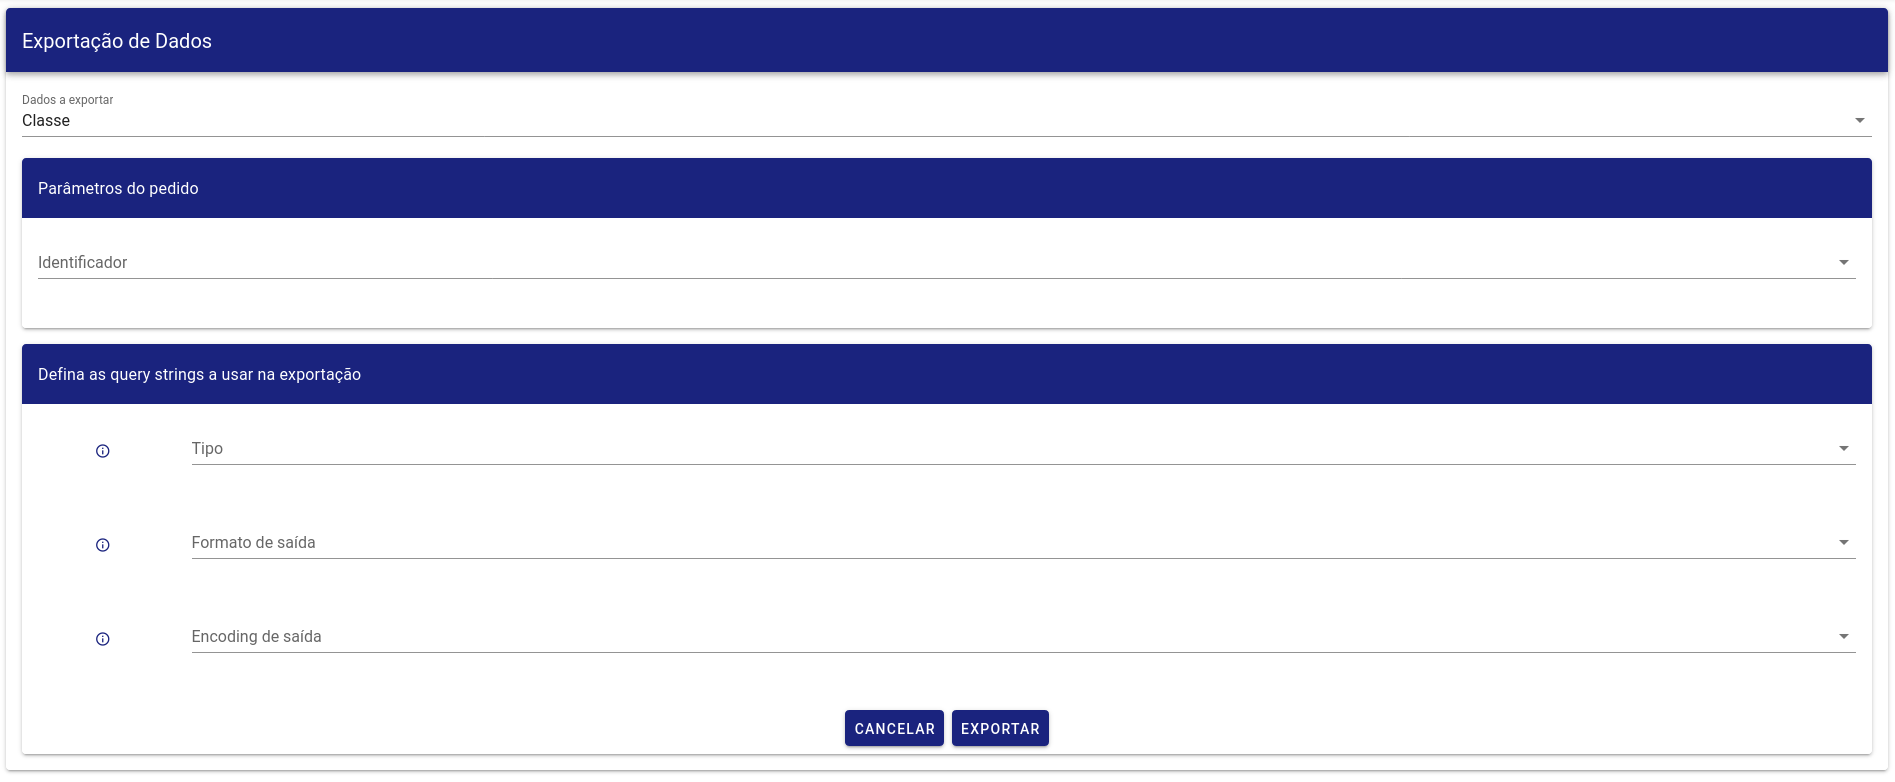
\includegraphics[width=0.9\textwidth]{img/paginaExportacao.png}
    \caption{Interface de exportação\label{fig:paginaExportacao}}
\end{figure}

Esta página de exportação está acessível em \url{https://clav.dglab.gov.pt/exportar}.

\section{Resumo}

Recapitulando, neste capítulo são inicialmente aprofundadas, no estado da arte, algumas bibliotecas disponíveis no \acrshort{npm} que têm como objetivo exportar de \acrshort{json} para \acrshort{xml} ou de \acrshort{json} para \acrshort{csv}. É por fim, investigado como poderá ser exportada a ontologia (exportação para \acrshort{rdf}) a partir do \textit{GraphDB}.

Já na secção da solução são apresentados as especificações das conversões a realizar bem como escolhidos que conversores serão usados enquanto que na secção da implementação são apresentados exemplos das conversões que os conversores realizam.
